\documentclass[a4paper]{article}
\usepackage[spanish]{babel}
\usepackage[utf8]{inputenc}
\usepackage{fancyhdr}
\usepackage{verbatim}
\usepackage{charter} % tipografia
%\usepackage{graphicx}
\usepackage[pdftex]{graphicx}
\usepackage{bm} % bold font in math mode
\usepackage{sidecap}
\usepackage{caption}
\usepackage{subcaption}
\usepackage{booktabs}
\usepackage{makeidx}
\usepackage{float}
\usepackage{amsmath, amsthm, amssymb}
\newtheorem{theorem}{Teorema}
\newtheorem{customthm}{Teorema}
\newtheorem{corollary}{Corolario}[theorem]
\newtheorem{proposition}[theorem]{Proposición}
\newtheorem{innercustomlemma}{Lemma}
\newenvironment{customlemma}[1]
  {\renewcommand\theinnercustomlemma{#1}\innercustomlemma}
  {\endinnercustomlemma}
\usepackage{amsfonts}
\usepackage{comment}
\usepackage{sectsty}
\usepackage{wrapfig}
\usepackage{listings}
\usepackage{hyperref} % links
\usepackage{algorithm} %http://www.ctan.org/pkg/algorithms
\usepackage{algorithmic}
\usepackage[usenames,dvipsnames]{xcolor}
\usepackage{pgfplots}
\usepackage{pgf-pie}
\usepackage{tabularx} % tablas copadas
% \usepackage{pgfplotstable}
% custom
\usepackage{color} % para snipets de codigo coloreados
\usepackage{fancybox} % para el sbox de los snipets de codigo
\definecolor{litegrey}{gray}{0.94}
% \newenvironment{sidebar}{%
% \begin{Sbox}\begin{minipage}{.85\textwidth}}%
% {\end{minipage}\end{Sbox}%
% \begin{center}\setlength{\fboxsep}{6pt}%
% \shadowbox{\TheSbox}\end{center}}
% \newenvironment{warning}{%
% \begin{Sbox}\begin{minipage}{.85\textwidth}\sffamily\lite\small\RaggedRight}%
% {\end{minipage}\end{Sbox}%
% \begin{center}\setlength{\fboxsep}{6pt}%
% \colorbox{litegrey}{\TheSbox}\end{center}}

%\newenvironment{codesnippet}{%
%\begin{Sbox}\begin{minipage}{\linewidth-2\fboxsep-2\fboxrule-4pt}\sffamily\small}%
%{\end{minipage}\end{Sbox}%
%\begin{center}%
%\colorbox{litegrey}{\TheSbox}\end{center}}

% \newenvironment{codesnippet}{\VerbatimEnvironment%
%   \noindent
%   %{\columnwidth-\leftmargin-\rightmargin-2\fboxsep-2\fboxrule-4pt}
%   \begin{Sbox}
%   \begin{minipage}{\linewidth-2\fboxsep-2\fboxrule-4pt}
%   \begin{Verbatim}
% }{%
%   \end{Verbatim}
%   \end{minipage}
%   \end{Sbox}%
%   \colorbox{litegrey}{\TheSbox}
% }

\newenvironment{codesnippet}{%
  \noindent
  %      {\columnwidth-\leftmargin-\rightmargin-2\fboxsep-2\fboxrule-4pt}
  \begin{Sbox}
  \begin{minipage}{\linewidth}
  \begin{lstlisting}
}{
  \end{lstlisting}
  \end{minipage}
  \end{Sbox}%
  \colorbox{litegrey}{\TheSbox}
}

\usepackage{fancyhdr}
\pagestyle{fancy}
%\renewcommand{\chaptermark}[1]{\markboth{#1}{}}
\renewcommand{\sectionmark}[1]{\markright{\thesection\ - #1}}
\fancyhf{}
\fancyhead[LO]{Sección \rightmark} % \thesection\
\fancyfoot[LO]{\small{Federico De Rocco, Jos\'e Massigoge, Leandro Anacondio}}
\fancyfoot[RO]{\thepage}
\renewcommand{\headrulewidth}{0.5pt}
\renewcommand{\footrulewidth}{0.5pt}
\setlength{\hoffset}{-0.8in}
\setlength{\textwidth}{16cm}
%\setlength{\hoffset}{-1.1cm}
%\setlength{\textwidth}{16cm}
\setlength{\headsep}{0.5cm}
\setlength{\textheight}{25cm}
\setlength{\voffset}{-0.7in}
\setlength{\headwidth}{\textwidth}
\setlength{\headheight}{13.1pt}
\renewcommand{\baselinestretch}{1.1} % line spacing

% \setcounter{secnumdepth}{2}
\usepackage{underscore}
\usepackage{kbordermatrix}% Matrix column labels
\usetikzlibrary{arrows,shapes}
\usepackage{tkz-graph}
\usepackage{caratula}
\usepackage{url}
\lstset{
    language=XML,
    basicstyle=\ttfamily,
    keywordstyle=\color{black}\ttfamily,
    stringstyle=\color{black}\ttfamily,
    commentstyle=\color{ForestGreen}\ttfamily,
    morecomment=[l][\color{magenta}]{\#},
    literate={á}{{\'a}}1 {ó}{{\'o}}1 {é}{{\'e}}1 {í}{{\'i}}1 {ú}{{\'u}}1 {Á}{{\'A}}1 {Í}{{\'I}}1 {É}{{\'E}}1 {Ú}{{\'U}}1 {Ó}{{\'O}}1 {\ \ }{{\ }}1,
  breaklines=true,
  tabsize=2
}

\DeclareUnicodeCharacter{2212}{-}

% *********************** %
\usepackage{tikz}
\usetikzlibrary{graphs}
\usetikzlibrary{calc}
\usetikzlibrary{arrows}
\usetikzlibrary{matrix}
% Otros
\usepackage{arrayjobx}
\usepackage{enumitem}
\usepackage{multicol}
\usepackage{natbib}
\usepackage{etoolbox}
\usepackage{listingsutf8}
\lstset{inputencoding=utf8/latin1}
\usepackage{fancyvrb}
\usepackage{pgfplotstable}
\usepackage{float}
\newcommand{\subscript}[2]{$#1 _ #2$}


% ******************************************************** %
\begin{document}
\thispagestyle{empty}
\materia{Teoría de Lenguajes}
\submateria{Segundo Cuatrimestre de 2016}
\titulo{Trabajo Práctico I}
\subtitulo{Grupo: Parsers para todos}
\integrante{Federico De Rocco}{408/13}{fede.183@hotmail.com}
\integrante{Jos\'e Massigoge}{954/12}{jmmassigoge@gmail.com}
\integrante{Leandro Anacondio}{487/07}{leandro.anacondio@gmail.com}
\maketitle
% no footer on the first page
\thispagestyle{empty}
\newpage

\tableofcontents

\newpage
\section{Introducción}
En el presente Trabajo Práctico diseñamos una gramática para el lenguaje \textit{Dibu} e implementamos sus analizador
léxico y su analizador sintáctico y semántico (parser). Utilizando estas herramientas creamos un programa que permite
traducir de \textit{Dibu} a \textit{SVG} y compilar dicha traducción, en caso de que sea válida. En los siguientes items
se describirán la gramática para el lenguaje, el lexer y el parser.


\newpage
\section{Gramática}
En la siguiente sección vamos a mostrar y describir la gramática construida para el lenguaje \textit{Dibu}, llamo a esta
gramática G:\\
\\
P $\rightarrow$ S newline P $\mid$ $\lambda$\\
S $\rightarrow$ id PARAMS\\
PARAMS $\rightarrow$  id = V PARAMS P $\mid$ id = V\\
V $\rightarrow$ num $\mid$ string $\mid$ (num, num) $\mid$ [ARRAY]\\
ARRAY $\rightarrow$ [num, num], ARRAY $\mid$ [num, num]\\
\\
\textit{G} = \{\{P, S, PARAMS, V, ARRAY\}, \{num, string, (, , , ), [, ], =, id, newline\}, Descripto por la gramática, P\}\\

Como se describe en el enunciado, el lenguaje \textit{Dibu} es una serie de instrucciones de la forma:\\
\\
IDENTIFICADOR PARAM1=V1, PARAM2=V2, ..., PARAMN=VN\\

Nuestra gramática consiste en cinco producciones. Comenzando con ARRAY la cual describe la secuencia de valores numericos
separados por una coma, la cual se utilizara en V para describir arreglos. La producción V que contiene las combinaciones
de terminales que se pueden esperar como valores de los parámetros (num, string, point, array).
PARAMS posee la serie de compuesta por: parámetro = valor. S describe una instrucción, con su nombre y parámetros. Y
finalmente P, describe la serie compuesta de las instrucciones descriptas en el no-terminal S. Con estas producciones se
puede ver con estos que nuestra gramática describe precisamente la serie de instrucciones de \textit{Dibu}. Se debe
aclarar que esta gramática no describe todas las restricciones de \textit{Dibu}, como por ejemplo que solo aparezca la
instrucción size una vez. Estas cuestriones se tratarán en el lexer y el parser.\\

Por otro lado tenemos el tipo de la gramática, para exponer esta información no realizaremos una demostración rigurosa
aunque si analizaremos la misma descartando en primera instancia que la gramática sea ambigua. Posteriormente reafirmaremos
en que tipos de gramáticas no se cuenta y el por qué.\\

Esta gramática no es LL(1) porque las producciones de PARAMS no cumplen con el
requerimiento de estas gramáticas(SD(PARAMS $\rightarrow$ id = V PARAMS P) $\cup$ SD(PARAMS $\rightarrow$ id = V)).\\

La gramática tampoco es LR(0). A continuación se mostrara el autómata correspondiente a la gramática, marcando los conflictos.\\


\includegraphics[scale=0.5]{imagenes/tleng.png}


No es SLR ya que los siguientes de PARAMS son \{newline, id\} por lo tanto no se resuelve el conflicto ya que hay un
shift/reduce provocado por el terminal id aunque si resuelve los demás conflictos.\\

Finalmente nuestra gramática es LR(1), observemos que el primer conflicto quedaría resuelto ya que solo haría reduce en
 \$, en el caso del segundo se resolvería de la misma forma. En el caso del tercero, en una producción anterior arrastraría
 el token newline y terminaría reduciendo por este, eliminando así el conflicto provocado por id. Por último tenemos el cuarto
similar al anterior en las producciones anteriores se los asociaría con el token ] el cual eliminaría el conflicto con la coma.


\newpage
\section{Lexer}
En esta sección vamos a explicar el analizador léxico implementado para la gramática descripta anteriormente. Al aplicar un
lexer sobre una cadena de caracteres este devolverá verdadero si la misma no contiene errores de carácter léxico como por
ejemplo caracteres que el lenguaje no reconoce. Para llevar a cabo este analizador contamos con una serie de tokens de
los cuales se da una descripción de sus posibles contenidos. Estos son:
\newline
\newline
\textbf{NUMBER}: Son todos los números compuestos por los caracteres numéricos del 0 al 9 y el punto. El lexer identifica el tipo
del valor numérico siendo estos enteros y de punto flotante de acuerdo a si el numero posee o no el punto. Esto se hace
para el posterior control de errores.\\
\textbf{Expresi\'on Regular}: $(0|..|9)^{+}(.(0|..|9)^{+})?$
\newline
\newline
\textbf{STRING}: Cadenas de caracteres entre comillas compuestas por las letras de la a a la z, incluidas mayúsculas, los números del
0 al 9 y los símbolos +,- y *.\\
\textbf{Expresi\'on Regular}: $"(a|..|z|A|..|Z|+|*|-)^{*}(a|..|z|A|..|Z|+|*|-|0|..|9)^{*}"$
\newline
\newline
\textbf{ID}: Igual que STRING pero sin las comillas.\\
\textbf{Expresi\'on Regular}: $(a|..|z|A|..|Z|+|*|-)^{*}(a|..|z|A|..|Z|+|*|-|0|..|9)^{*}$
\newline
\newline
\textbf{LPAREN}: El carácter $[$.\\
\newline
\textbf{RPAREN}: El carácter $]$.\\
\newline
\textbf{LBRACKET}: El carácter $($.\\
\newline
\textbf{RBRACKET}: El carácter $)$.\\
\newline
\textbf{COMMA}: El carácter $,$.\\
\newline
\textbf{EQUALS}: El carácter $=$.\\
\newline
\textbf{NEWLINE}: El salto de linea. Este tiene la particularidad de que aumenta en una linea el largo del texto, esto se
utiliza para detectar la posición de los errores.\\
\newline
\textbf{IGNORE}: El carácter vacío.\\
\newline
\textbf{ERROR}: Este aparece cuando se encuentra un token desconocido. En consecuencia se guarda la linea, valor, posición y
tipo de valor para el error. Con este último cumplimos que si la cadena es inválida se detectara el error y se informará de él.\\
\newline
Como se puede ver con esta serie de tokens y sus respectivas implementaciones podemos describir todos los posibles no terminales y terminales
necesarios para nuestra gramática. Quedan todavía restricciones como por ejemplo que ID solamente puede tener como valores a los
identificadores de las instrucciones.\\


\newpage
\section{Parser}
En esta secci�n vamos a explicar el analizador sint�ctico o parser implementado . El an�lisis sint�ctico convertir� el texto de entrada 
en el �rbol de derivaci�n pertinente. A partir de ello hacemos el an�lisis de las sentencias, utilizando estructuras auxiliares para
cumplir posteriormente con el requerimiento de la generaci�n del texto de salida (en formato svg).
La idea general fue definir una funci�n que represente cada una de las producciones de nuestra, y dentro de cada una ir manipulando la 
informaci�n para luego generar el output requerido.
Como atributos utilizamos lineno y lexpos para detallar el n�mero de l�nea y posici�n respectivamente, mientras que el atributo value nos devuelve el valor.
Como estructuras auxiliares utilizamos un diccionario y una lista. El primero representa los par�metros obligatorios de cad una de las
figuras, lo utilizamos dentro de la produccion STATE para chequear que todos los par�metros obligatorios est�n dentro de la cadena de entrada
para cada figura en particular. El segundo es simplemente una lista donde iremos acumulando las distintas figuras que se fueron generando, teniendo 
en cuenta que nuestro parser es bottom-up, las figuras se iran generando a partir de las hojas y una vez que se llegue a la producci�n inicial, tendremos
la lista llena de las figuras que debemos imprimir.
Agregamos una funci�n que hiciera las veces de producci�n inicial solo a fines pr�cticos, para poder generar el lienzo final, e ir 
agregando las figuras que posteriormente dibujaremos.
A continuaci�n haremos un an�lisis de cada una de esas funciones para explicar cu�l es su rol.

P_START: genera el lienzo llamando a la funci�n Scene (definida en la clase helper.py) y luego le agrega las figuras de la lista al mismo.
Tambi�n chequea que no se haya llamado a la funci�n size mas de una vez.

P_PROGRAM_EMPTY: representa al programa que se genera a partir de la producci�n P $\mid$ $\lambda$\\

P_PROGRAM_NONEMPTY: representa al programa que se genera a partir de la producci�n P $\rightarrow$ S newline P

P_STATE: Es la funci�n m�s compleja del parser. Primero chequea que el token sea size, si lo es, se revisa que tenga el height y width que son los par�metros requeridos.
Si el token no es size estamos ante la producci�n para generar una figura, por ello, se guarda los parametros recolectados por los nodos hijos en una variable,
 e inicializa la figura como objeto (correspondiente al nombre de la misma, dentro de una funci�n auxiliar).
Si la generaci�n no lanza una excepci�n, va completando los atributos requeridos por esa figura y la agrega a la lista de resultados. Si no se genera bien la figura o si
los par�metros son incorrectos se lanza la excepci�n correspondiente.

P_PARAMS_NONRECURSIVE: Representa la asignaci�n de un valor a un par�metro sin recursi�n, es decir es el �ltimo de la lista o es �nico. Dentro de esta funci�n se agrega 
el n�mero de l�nea, posici�n y valor del par�metro al diccionario de par�metros.

P_PARAMS_RECURSIVE: Representa la seguidilla de par�metros separados por coma. Chequea que no haya repetidos y los va agregando a la lista de par�metros.

P_VALOR_NUMBER: Realiza la asignaci�n de un valor a un par�metro de tipo num�rico.

P_VALOR_STRING: Realiza la asignaci�n de un valor a un par�metro de tipo string.

P_VALOR_POINT: Realiza la asignaci�n de un valor a un par�metro de tipo punto, es decir dos n�meros separados por coma.

P_VALOR_ARRAY: Realiza la asignaci�n de un valor a un par�metro de tipo arreglo.

P_ARRAY_ELEMENT: Representa el array con un �nico elemento, o el elemento final de un arreglo.

P_ARRAY_RECURSIVE: Genera un nuevo elemento en un array y lo appendea a los elementos que siguen en la producci�n

P_ERROR: Define los errores sint�cticos que ocurrieron. A partir del token genera el mensaje correspondiente.




%\newpage
%\section{Requerimientos de Software}
%<<<<<<< HEAD
Requerimientos m\'inimos:
- Python 2.7.*
- Ply 3.9

Instrucciones de uso:

Para generar el svg de salida debe ejecutarse la siguiente linea de comando (situado sobre el directorio src/dibu):
-python parser.py \"archivo de entrada\" \"nombre de imagen\".

El archivo de entrada debe contener el c�digo de la imagen que se quiere generar, y el nombre de la imagen ser\'a el nombre de la misma.


\newpage
\section{Test}
A continuación mostramos los resultados obtenidos de realizar test de las diversas figuras, especificando cual era el código \textit{Dibu} de entrada, el código \textit{SVG} de salida y la imagen generada.

\subsection{\textbf{Figura:} Rectangle}

Código \textit{Dibu} de entrada:

\begin{lstlisting}
  size height=400, width= 1200
  rectangle size=(398, 1198), upper_left=(1,1), fill="none", stroke="blue", stroke-width=2
  rectangle upper_left=(400,100), fill="yellow", size=(200, 400), stroke-width=10, stroke="navy"
\end{lstlisting}

Código \textit{SVG} de salida:

\begin{lstlisting}
  <?xml version="1.0"?>
  <svg height="400" width="1200" >
   <g style="fill-opacity:1.0; stroke:black;
    stroke-width:1;">
    <rect x="1" y="1" height="398"
      width="1198" style="fill:none;stroke:blue;stroke-width:2" />
    <rect x="400" y="100" height="200"
      width="400" style="fill:yellow;stroke:navy;stroke-width:10" />
   </g>
  </svg>
\end{lstlisting}

\begin{figure}[H]
\centering

\includegraphics[width=150mm]{imagenes/rectangle.jpg}
\caption{Imagen generada - Figura Rectangle}
\end{figure}

\subsection{\textbf{Figura:} Line}

Código \textit{Dibu} de entrada:

\begin{lstlisting}
  size width=1200, height=400
  rectangle size=(398, 1198), upper_left=(1,1), fill="none", stroke="blue", stroke-width=2
  line from=(100,300), to=(300,100), stroke-width=5, stroke="green"
  line from=(300,300), to=(500,100), stroke-width=10, stroke="green"
  line from=(500,300), to=(700,100), stroke-width=15, stroke="green"
  line from=(700,300), to=(900,100), stroke-width=20, stroke="green"
  line from=(900,300), to=(1100,100), stroke-width=25, stroke="green"
\end{lstlisting}

Código \textit{SVG} de salida:

\begin{lstlisting}
  <?xml version="1.0"?>
  <svg height="400" width="1200" >
   <g style="fill-opacity:1.0; stroke:black;
    stroke-width:1;">
    <rect x="1" y="1" height="398"
      width="1198" style="fill:none;stroke:blue;stroke-width:2" />
    <line x1="100" y1="300" x2="300" y2="100" style="fill:black;stroke:green;stroke-width:5"/>
    <line x1="300" y1="300" x2="500" y2="100" style="fill:black;stroke:green;stroke-width:10"/>
    <line x1="500" y1="300" x2="700" y2="100" style="fill:black;stroke:green;stroke-width:15"/>
    <line x1="700" y1="300" x2="900" y2="100" style="fill:black;stroke:green;stroke-width:20"/>
    <line x1="900" y1="300" x2="1100" y2="100" style="fill:black;stroke:green;stroke-width:25"/>
   </g>
  </svg>
\end{lstlisting}


\begin{figure}[H]
\centering

\includegraphics[width=150mm]{imagenes/line.jpg}
\caption{Imagen generada - Figura Linea}
\end{figure}

\subsection{\textbf{Figura:} Circle}

Código \textit{Dibu} de entrada:

\begin{lstlisting}
  size width=1200, height=400
  rectangle size=(398, 1198), upper_left=(1,1), fill="none", stroke="blue", stroke-width=2
  circle center=(600, 200), fill="red", stroke="blue", stroke-width=10, radius=100
\end{lstlisting}

Código \textit{SVG} de salida:

\begin{lstlisting}
  <?xml version="1.0"?>
  <svg height="400" width="1200" >
   <g style="fill-opacity:1.0; stroke:black;
    stroke-width:1;">
    <rect x="1" y="1" height="398"
      width="1198" style="fill:none;stroke:blue;stroke-width:2" />
    <circle cx="600" cy="200" r="100"
      style="fill:red;stroke:blue;stroke-width:10"  />
   </g>
  </svg>
\end{lstlisting}

\begin{figure}[H]
\centering

\includegraphics[width=150mm]{imagenes/circle.jpg}
\caption{Imagen generada - Figura Circulo}
\end{figure}

\subsection{\textbf{Figura:} Ellipse}

Código \textit{Dibu} de entrada:

\begin{lstlisting}
  size width=1200, height=400
  rectangle size=(398, 1198), upper_left=(1,1), fill="none", stroke="blue", stroke-width=2
  ellipse center=(300, 200), fill="red", ry=100, rx=250
  ellipse ry=100, fill="none", rx=250, center=(900, 200), stroke="blue", stroke-width=20
\end{lstlisting}

Código \textit{SVG} de salida:

\begin{lstlisting}
  <?xml version="1.0"?>
  <svg height="400" width="1200" >
   <g style="fill-opacity:1.0; stroke:black;
    stroke-width:1;">
    <rect x="1" y="1" height="398"
      width="1198" style="fill:none;stroke:blue;stroke-width:2" />
    <ellipse cx="300" cy="200" rx="250" ry="100"
      style="fill:red;stroke:none;stroke-width:1"/>
    <ellipse cx="900" cy="200" rx="250" ry="100"
      style="fill:none;stroke:blue;stroke-width:20"/>
   </g>
  </svg>
\end{lstlisting}

\begin{figure}[H]
\centering

\includegraphics[width=150mm]{imagenes/ellipse.jpg}
\caption{Imagen generada - Figura Elipse}
\end{figure}

\subsection{\textbf{Figura:} Polyline}

Código \textit{Dibu} de entrada:

\begin{lstlisting}
  size width=1200, height=400
  rectangle size=(398, 1198), upper_left=(1,1), fill="none", stroke="blue", stroke-width=2
  polyline points=[(50,375), (150,375), (150,325), (250,325), (250,375), (350,375), (350,250), (450,250), (450,375), (550,375), (550,175), (650,175), (650,375), (750,375), (750,100), (850,100), (850,375), (950,375), (950,25), (1050,25), (1050,375), (1150,375)], stroke="blue", stroke-width=10, fill="none"
\end{lstlisting}

Código \textit{SVG} de salida:

\begin{lstlisting}
  <?xml version="1.0"?>
  <svg height="400" width="1200" >
   <g style="fill-opacity:1.0; stroke:black;
    stroke-width:1;">
    <rect x="1" y="1" height="398"
      width="1198" style="fill:none;stroke:blue;stroke-width:2" />
  <polyline points=" 50,375 150,375 150,325 250,325 250,375 350,375 350,250 450,250 450,375 550,375 550,175 650,175 650,375 750,375 750,100 850,100 850,375 950,375 950,25 1050,25 1050,375 1150,375"
  style="fill:none;stroke:blue;stroke-width:10"/>
   </g>
  </svg>
\end{lstlisting}

\begin{figure}[H]
\centering
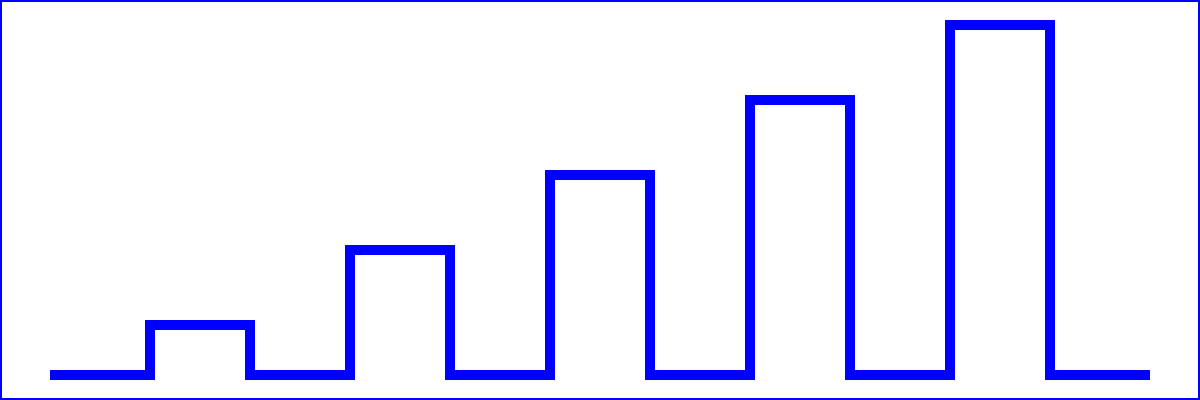
\includegraphics[width=150mm]{imagenes/polyline.jpg}
\caption{Imagen generada - Figura Polyline}
\end{figure}

\subsection{\textbf{Figura:} Polygon}

Código \textit{Dibu} de entrada:

\begin{lstlisting}
  size width=1200, height=400
  rectangle size=(398, 1198), upper_left=(1,1), fill="none", stroke="blue", stroke-width=2
  polygon fill="red", stroke="blue", stroke-width=10, points=[(350,75), (379,161), (469,161), (397,215), (423,301), (350,250), (277,301), (303,215), (231,161), (321,161)]
  polygon fill="lime", stroke="blue", stroke-width=10, points=[(850,75), (958,137.5), (958,262.5), (850,325), (742,262.6), (742,137.5)]
\end{lstlisting}

Código \textit{SVG} de salida:

\begin{lstlisting}
  <?xml version="1.0"?>
  <svg height="400" width="1200" >
   <g style="fill-opacity:1.0; stroke:black;
    stroke-width:1;">
    <rect x="1" y="1" height="398"
      width="1198" style="fill:none;stroke:blue;stroke-width:2" />
  <polygon points=" 350,75 379,161 469,161 397,215 423,301 350,250 277,301 303,215 231,161 321,161"
  style="fill:red;stroke:blue;stroke-width:10"/>
  <polygon points=" 850,75 958,137 958,262 850,325 742,262 742,137"
  style="fill:lime;stroke:blue;stroke-width:10"/>
   </g>
  </svg>
\end{lstlisting}


\begin{figure}[H]
\centering

\includegraphics[width=150mm]{imagenes/polygon.jpg}
\caption{Imagen generada - Figura Poligono}
\end{figure}

\newpage

\subsection{Errores Semánticos}
Otra de las cuestiones que nos pareció importante testear es la capacidad del parser de detectar errores semánticos. A partir del enunciado, concluimos que podrían darse los siguientes errores de esta índole:
\begin{enumerate}
  \item \textbf{Dos o mas usos de la sentencia Size.}
  \item \textbf{Nombre de figura invalida.}
  \item \textbf{Parámetro invalido.}
  \item \textbf{Ausencia de parámetros obligatorios.}
  \item \textbf{Parámetros repetidos.}
\end{enumerate}

Propusimos los siguientes test para testear esta característica:
\begin{enumerate}
  \item \textbf{Dos o mas usos de la sentencia Size.}

  Código \textit{Dibu} de entrada:

  \begin{lstlisting}
    size width=1200, height=400
    rectangle upper_left=(1,1), fill="none", stroke="blue", stroke-width=2, size=(200, 200)
    size height=400, width=200
    size height=800, width=800
    rectangle upper_left=(50,50), fill="none", stroke="red", stroke-width=2, size=(500, 800)
  \end{lstlisting}

  Texto emitido en el stdout:

  \begin{lstlisting}
    Semantic error: Dos o Mas Size
    line: 3
    position: 116
  \end{lstlisting}

  \item \textbf{Nombre de figura invalida.}

  Código \textit{Dibu} de entrada:

  \begin{lstlisting}
    cuadrado size=200, fill="red"
    rectangle upper_left=(1,1), fill="none", stroke="blue", stroke-width=2, size=(200, 200)
  \end{lstlisting}

  Texto emitido en el stdout:

  \begin{lstlisting}
    Semantic error: Figura Invalida
    line: 1
    position: 9
  \end{lstlisting}

  \item \textbf{Parámetro invalido.}

  Código \textit{Dibu} de entrada:

  \begin{lstlisting}
    line from=(100,300), to=(300,100), stroke-width=5, stroke="green"
    line from=(300,300), to=(500,100), stroke-width=10, stroke="green", rotate=(90,90)
  \end{lstlisting}

  Texto emitido en el stdout:

  \begin{lstlisting}
    Semantic error: Parametro Invalido
    line: 2
    position: 71
  \end{lstlisting}

  \item \textbf{Ausencia de parámetros obligatorios.}

  Código \textit{Dibu} de entrada:

  \begin{lstlisting}
    line to=(300,100), stroke-width=5, stroke="green"
    line from=(300,300), to=(500,100), stroke-width=10, stroke="green"
  \end{lstlisting}

  Texto emitido en el stdout:

  \begin{lstlisting}
    Semantic error: Faltan Parametros obligatorios
    line: 1
    position: 5
  \end{lstlisting}

  \item \textbf{Parámetros repetidos.}

  Código \textit{Dibu} de entrada:

  \begin{lstlisting}
    line from=(100,100), to=(300,100), stroke-width=5, stroke="green", stroke-width=3
    line from=(300,300), to=(500,100), stroke-width=10, stroke="green"
  \end{lstlisting}

  Texto emitido en el stdout:

  \begin{lstlisting}
    Semantic error: Parametros repetidos
    line: 1
    position: 35
  \end{lstlisting}

\end{enumerate}


\newpage
\section{Conclusiones}
El desaf\'io de desarrollar un lenguaje desde su inicio, resulta interesante para comprender como se definen las reglas sint\'acticas y sem\'anticas que conforman la estructura del mismo.
A lo largo del trabajo tuvimos que repensar varias veces incluso los puntos que parec\'ian m\'as simples, como ser la definici\'on de la gram\'atica y el impacto que generaba cada decisi\'on tomada.
En el aspecto meramente implementativo tambi\'en modificamos sobre la marcha las estructuras utilizadas y la forma en que utiliz\'abamos los datos, en un proceso iterativo.
Todo lo antes dicho lleva a pensar que incluso el desarrollo de lenguajes peque\~nos, conlleva un gran trabajo y cada decisi\'on tomada impacta de forma directa en las etapas siguientes.


\end{document}
